% Evaluation 2 report. Retains the Evaluation 1 section flow and authors.
% Compile from this directory: latexmk -pdf main.tex
\documentclass[conference,a4paper]{IEEEtran}
\usepackage[T1]{fontenc}
\usepackage{cite}
\usepackage{amsmath,amssymb}
\usepackage{graphicx}
\usepackage{booktabs,array,tabularx}
\usepackage{xcolor}
\usepackage{tikz}
\usetikzlibrary{arrows.meta,positioning,shapes.geometric,fit}
\usepackage{url}
\usepackage[hidelinks]{hyperref}
\usepackage{balance}
\usepackage{placeins}
\graphicspath{{figures/}}
\newcolumntype{P}[1]{>{\raggedright\arraybackslash}p{#1}}
\newcolumntype{Y}{>{\raggedright\arraybackslash}X}
% Generated from reports/multimodal-real-v2/comparison.csv
\newcommand{\CascadeAccuracy}{85.48}
\newcommand{\CascadeRecall}{88.16}
\newcommand{\CascadeFone}{0.810}
\newcommand{\FusionRecall}{88.82}
\newcommand{\RecallGap}{0.66}
\newcommand{\CpuSaving}{15.08}
\newcommand{\CascadeCpu}{14.24}
\newcommand{\FusionCpu}{16.77}
\newcommand{\RecallGain}{13.82}

\newcommand{\system}{Pulsepoint}
\newcommand{\pct}{\%}
\newcommand{\RR}{\mathrm{RR}}
\hyphenation{electro-dermal physio-logical multi-modal}
\setlength{\emergencystretch}{1em}

\title{Quality-Aware Adaptive Multimodal Stress Detection Using Wearable Sensor Data for Edge AIoT}
\author{
\IEEEauthorblockN{Saanvi Bansal}
\IEEEauthorblockA{Registration No.: 240953564}
\and
\IEEEauthorblockN{Shobit Hegde}
\IEEEauthorblockA{Registration No.: 240953556}
\and
\IEEEauthorblockN{Pranav Gaddam}
\IEEEauthorblockA{Registration No.: 240953548}
}
\begin{document}
\maketitle

\begin{abstract}
Wearable healthcare systems require useful predictions despite constrained processing resources and imperfect physiological measurements. This work develops a quality-aware adaptive stress-classification pipeline that first processes electrocardiogram (ECG), requests electrodermal activity (EDA) and respiration when additional evidence is needed, and uses an independent alternate expert when ECG fails. Unusable evidence produces an explicit rejection. The implementation extends an earlier edge-based AIoT proposal into a local, reproducible software prototype. Fifteen-subject leave-one-subject-out evaluation on WESAD scores 434 eligible, nonoverlapping 60-second replay windows under eleven clean and corruption scenarios. The revised cascade achieves \CascadeAccuracy\pct{} accuracy, \CascadeRecall\pct{} all-window stress recall and an F1-score of \CascadeFone{} at full clean coverage. Relative to always-on fusion, mean processing CPU time falls by \CpuSaving\pct{}, with a \RecallGap{}-percentage-point recall reduction in the held-out training-procedure evaluation. Under ECG flatline, alternate inference retains 85.25\pct{} accuracy and 0.787 F1 at full coverage. A separate benchmark of the final fitted artifact shows no CPU saving on its sampled replay workload. The results demonstrate a useful laboratory tradeoff and ECG-failure resilience while exposing policy instability, amplitude sensitivity and remaining deployment limitations.
\end{abstract}

\begin{IEEEkeywords}
AIoT, wearable stress detection, edge-oriented inference, multimodal fusion, signal quality, adaptive routing, WESAD.
\end{IEEEkeywords}

\section{Introduction}
The Internet of Things (IoT) connects sensing devices, communication interfaces and computational services so that physical measurements can support applications. In healthcare, wearable sensors provide repeated observations without requiring the user to manually record every measurement. A practical system must turn these streams into information that can be interpreted by a user. The usefulness of a wearable application therefore depends on its complete sensing-to-decision pipeline, including signal quality, processing cost and the handling of missing information.

Artificial Intelligence of Things (AIoT) adds learned inference to this pipeline. A conventional sensing application can collect and display measurements, whereas an AIoT application can classify a measured pattern and decide what additional processing is warranted. This distinction motivates the present work: the system should decide both \emph{what state the available measurements suggest} and \emph{whether the available evidence is sufficient}. Treating every received window as equally reliable would hide a central difficulty of wearable monitoring.

Stress recognition provides a concrete setting for studying these decisions. ECG, EDA and respiration offer complementary measurements of physiological activity. WESAD provides synchronized recordings from wearable devices and establishes a public benchmark for stress and affect recognition~\cite{schmidt2018}. However, a dataset label describes an experimental condition; a prediction from a short window is not a diagnosis of an individual's psychological or medical state. This report consequently evaluates baseline-versus-stress classification under the dataset's condition labels and keeps the clinical interpretation outside the experimental claim.

Local processing is attractive because a basic prediction need not depend on a remote inference service. Wearable and edge-computing research examines several ways to place inference near the data source~\cite{pereira2024,mitro2023}. Nevertheless, moving software onto a local host does not itself prove improved energy efficiency or suitability for a microcontroller. Feature extraction, quality inspection, model execution and routing all consume computation. An efficiency comparison must measure those stages together and distinguish host timing from measurements on a physical target device.

\begin{figure}[t]
\centering
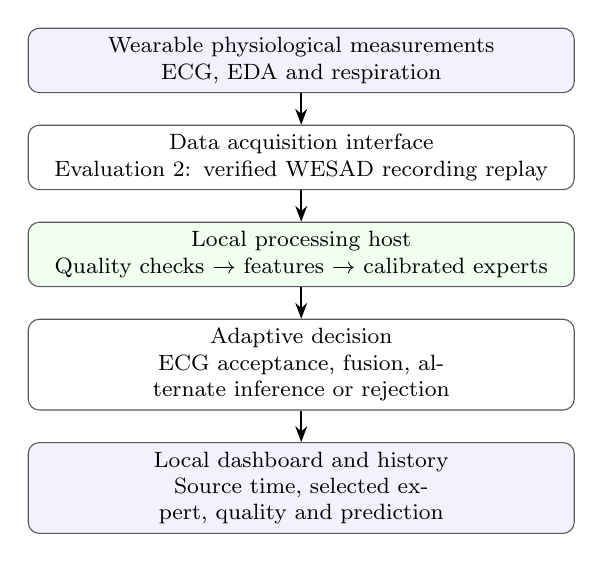
\begin{tikzpicture}[node distance=4mm,box/.style={draw=black!65,rounded corners,align=center,font=\footnotesize,text width=6.7cm,minimum height=7mm},arr/.style={-{Stealth[length=2mm]},thick}]
\node[box,fill=blue!5] (sense) {Wearable physiological measurements\\ECG, EDA and respiration};
\node[box,below=of sense] (source) {Data acquisition interface\\Evaluation 2: verified WESAD recording replay};
\node[box,below=of source,fill=green!6] (edge) {Local processing host\\Quality checks $\rightarrow$ features $\rightarrow$ calibrated experts};
\node[box,below=of edge] (decision) {Adaptive decision\\ECG acceptance, fusion, alternate inference or rejection};
\node[box,below=of decision,fill=blue!5] (ui) {Local dashboard and history\\Source time, selected expert, quality and prediction};
\draw[arr] (sense)--(source);\draw[arr] (source)--(edge);\draw[arr] (edge)--(decision);\draw[arr] (decision)--(ui);
\end{tikzpicture}
\caption{Application-specific AIoT architecture. The implemented acquisition interface replays recorded data; live wearable connectivity and physical edge deployment remain future work. The inference path has no cloud dependency.}
\label{fig:context}
\end{figure}

Always processing every modality is straightforward but can perform unnecessary work on windows that a smaller expert can resolve. Always using ECG alone is cheaper in some settings but loses access to complementary evidence when ECG is unreliable. Adaptive multimodal systems investigate this tension~\cite{amser2022}. Their existence also means that adaptivity itself is established prior art. The contribution of this project is a specific, inspectable integration of calibrated experts, quality and confidence gates, explicit rejection, chronological replay and participant-held-out cost and failure analysis.

Three challenges shape the design. First, confidence is a learned quantity and can be unreliable for a new participant or a shifted signal. A high score does not prove that the input remains in the model's training distribution. Second, missing ECG should not automatically imply baseline: another supported expert must make the decision, or the system must decline to classify. Third, a cascade only saves work when sufficiently many windows avoid the additional path. Computing ECG and subsequently invoking fusion on almost every window can remove the intended saving.

The research question is therefore: \emph{Can quality-aware adaptive multimodal processing retain useful stress recall while reducing processing cost and maintaining operation under sensor failure?} Figure~\ref{fig:context} places that question within an AIoT workflow. The study evaluates the question through measured comparisons, rather than assuming that edge-oriented design guarantees all three benefits simultaneously. Classification quality, accepted coverage and processing cost are reported together so that a system cannot appear accurate simply by rejecting difficult stress windows.

\subsection{Continuity from Evaluation 1}
Evaluation 1 proposed edge-based stress monitoring with wearable signals, lightweight classifiers, optional cloud interaction and an eventual user display. Evaluation 2 retains that application, problem framing, literature basis, research gap and architecture. The implementation narrows the scope to synchronized chest ECG, EDA and respiration and replaces the broad list of possible models with three calibrated experts selected from logistic regression, SVM and bounded forest candidates. KNN and a compact CNN were considered in the earlier proposal but are not reported as implemented experiments. Adaptive routing and failure analysis provide the completed technical extension.

\subsection{Contributions}
The completed contributions are: (i) a reproducible multimodal pipeline with source-interval provenance and independently calibrated experts; (ii) separate rules for requesting extra evidence and accepting a final decision, including modality-aware fallback; (iii) a shared local runtime used for evaluation, replay and the dashboard; and (iv) fifteen participant-held-out folds across eleven waveform scenarios, with baselines, ablations, coverage, participant uncertainty and processing measurements. The results include both improvements and failure cases. In particular, the final fitted model's benchmark is separated from the held-out procedure so that a favorable cross-validation result is not attributed to an untested deployment instance.

\section{Literature Survey}
The literature retained from Evaluation 1 covers public wearable data, edge healthcare and privacy-aware stress learning. The revised survey additionally examines adaptive sensing and selective classification because these directly constrain the project's originality claim. Conference papers and journal articles are compared by their research question, architecture, data, method, reported outcome and practical limitation. Published scores are described in their original context and are not pooled with the present experiment.

\subsection{Public Multimodal Stress Benchmark}
Schmidt et al.~\cite{schmidt2018} introduced WESAD as a multimodal wearable stress and affect dataset. Their chest and wrist recordings support classical feature-based benchmarking and comparison of sensor locations. The paper reports binary accuracy up to approximately 93\pct{} and three-class accuracy up to approximately 80\pct{} under its own protocol. Its principal strength is a shared experimental resource; its laboratory setting limits claims about unconstrained everyday use. The present project adopts the recordings, not the assumption that a published score transfers to different labels, windows or splits. Its baseline-versus-stress replay task excludes mixed and unsupported conditions from binary scoring, so direct numerical ranking against the original benchmark would be inappropriate.

\subsection{Edge Computing and Wearable Healthcare: Journal Evidence}
Pereira et al.~\cite{pereira2024} systematically mapped machine learning, edge computing and wearable healthcare. Their review screened 171 studies and focused on 28 selected articles, identifying varied applications, models and edge platforms. This journal contribution supports examining architecture and deployment constraints alongside accuracy. Its strength is breadth across the field; its heterogeneous tasks and evaluation methods do not provide one directly comparable stress-classification benchmark. For this project, the implication is methodological: local execution, processing stages and device assumptions should be stated explicitly, and measurements from different applications should not be treated as interchangeable evidence.

Mitro et al.~\cite{mitro2023} presented an AI-enabled wristband for vital-sign and stress monitoring, including model execution on the wearable's microcontroller. The architecture connects sensing, embedded inference and a practical monitoring application. Its reported hardware execution is important because it moves beyond an offline classifier. However, hardware-specific results cannot be assigned to a desktop implementation with different signals and processing. Relative to that work, the present study offers a software and failure-analysis prototype; a real device experiment remains a separate requirement. This distinction prevents local host timing from being presented as measured wearable energy or microcontroller latency.

\subsection{Personalized, Centralized and Federated Stress Learning}
Fauzi et al.~\cite{fauzi2022} compared individual, centralized and federated learning for smartwatch-based stress detection using WESAD. The journal study examines how learning organization and differences among users affect classification. Its comparison found advantages for individual models in the investigated setting, illustrating the importance of participant variation. Federated learning offers a distributed training architecture but introduces concerns different from the runtime decision of whether to request another modality. The present project does not implement federation or user onboarding. Instead, it evaluates unseen participants and explicitly separates fitting, calibration and policy selection. Personalization would require a future protocol in which adaptation data are excluded from the scored evaluation interval.

\subsection{Adaptive Multimodal Sensing}
Naeini et al.~\cite{amser2022} proposed AMSER, an adaptive multimodal sensing framework for energy-efficient and resilient eHealth. Its architecture changes feature or modality configurations and selects suitable models in response to sensing conditions. The work demonstrates this approach through pain and stress case studies and reports a resilience--resource tradeoff. This is direct prior art for the general adaptive-sensing idea. The present contribution is consequently narrower: an ECG-first calibrated cascade with separate exit and acceptance thresholds, explicit unavailable-evidence handling and a reproducible WESAD evaluation. AMSER's sensing-energy results are not reproduced here; processing already acquired recordings establishes neither sensor scheduling nor battery savings.

\subsection{Selective Classification and Confidence}
Geifman and El-Yaniv~\cite{geifman2017} formalized selective classification in which a predictor can reject uncertain inputs, exposing a tradeoff between accepted coverage and risk. The work concerns neural-network classification rather than wearable sensor architecture, but it supplies a useful conceptual basis for rejection. Its implication here is that accepted-only accuracy must be accompanied by coverage. A system that declines to answer on most stress windows may have attractive accepted accuracy but poor operational detection. This project therefore reports all-window stress recall, counting rejected stress windows as undetected, while keeping accepted-decision metrics separate. It does not claim a formal selective-risk guarantee under physiological distribution shift.

\begin{table*}[t]
\centering\small
\caption{Critical comparison of the literature and the implemented project. Three retained studies are journal articles. Outcomes refer to each study's own setting; they are not a common leaderboard.}
\label{tab:literature}
\begin{tabularx}{\textwidth}{P{2.15cm}P{2.8cm}P{3.0cm}Y}\toprule
Study / venue type & Problem, architecture and method & Data and reported outcome & Strength, limitation and implication for this project\\\midrule
Schmidt et al.~\cite{schmidt2018}, conference & Wearable stress/affect benchmark; chest/wrist feature-based ML & WESAD laboratory recordings; binary accuracy up to about 93\pct{} in the original protocol & Common dataset; protocol and deployment differences prevent direct score transfer.\\
Pereira et al.~\cite{pereira2024}, journal review & Mapping ML across wearable/edge healthcare architectures & Literature corpus; 28 selected studies from 171 screened & Broad architectural perspective; heterogeneous metrics require task-specific evaluation.\\
Mitro et al.~\cite{mitro2023}, journal & Wearable vital-sign/stress system with embedded inference & Wristband sensing and demonstrated MCU execution & Hardware realization; its deployment evidence cannot be inherited by host software.\\
Fauzi et al.~\cite{fauzi2022}, journal & Individual, centralized and federated smartwatch stress learning & WESAD; learning-strategy comparison highlights user variation & Privacy/training comparison; runtime modality selection is a separate question.\\
Naeini et al.~\cite{amser2022}, conference & Adaptive feature/modality configurations and model selection & Pain and stress case studies; resource/resilience evaluation & Establishes adaptive-sensing prior art; energy experiments differ from processing-only measurements.\\
Geifman and El-Yaniv~\cite{geifman2017}, conference & Selective prediction with rejection & Neural classification; risk--coverage analysis & Makes rejection explicit; no automatic reliability guarantee for corrupted biosignals.\\
This work, Evaluation 2 & Calibrated ECG/alternate/fusion experts; quality-aware local routing & WESAD; 15 outer folds, 11 waveform scenarios, recorded CPU and coverage & Integrated, reproducible stress-specific study; limited cohort, host-only timing and unstable artifact efficiency.\\\bottomrule
\end{tabularx}
\end{table*}

\subsection{Comparative Findings}
The studies address complementary layers: WESAD enables shared data analysis, the edge-healthcare mapping frames implementation constraints, the wristband demonstrates physical integration, federated learning examines training organization, AMSER establishes adaptive sensing, and selective classification explains rejection. A practical implementation still needs to make these concerns inspectable in one experimental pipeline. The opportunity addressed here is not the absence of multimodal or edge methods. It is the specific evaluation of calibrated routing, usable coverage, quality-based fallback and measured processing cost on matched held-out source windows. Table~\ref{tab:literature} identifies both the foundation provided by prior work and the narrower scope of this implementation.

The literature also changes how the results should be interpreted. A high classification score alone does not demonstrate a complete wearable system; an edge-oriented diagram alone does not demonstrate a resource saving; and a rejection mechanism alone does not establish reliable stress monitoring. The evaluation must expose the complete decision path. This motivates retaining negative results, including amplitude sensitivity and the discrepancy between fold-level efficiency and the final artifact's benchmark, as part of the research finding.

\section{Research Gap}
Evaluation 1 identified the need to connect wearable stress classification with lightweight local processing. The implemented study makes that gap more specific: a stress-monitoring runtime must decide when a low-cost expert is sufficient, when additional modalities are useful and when the available measurements cannot support a prediction. The decision must remain meaningful under missing or damaged sensors and must be assessed against the work required by full fusion.

Adaptive sensing already exists~\cite{amser2022}. The gap addressed in this project is an implementation and evaluation gap: jointly documenting quality-aware escalation, calibrated class-specific exit rules, alternate-sensor fallback, explicit rejection and source-time event state, while reporting both accuracy-related quantities and processing cost on the same held-out inputs. The study does not establish publication-level uniqueness over every prior policy. It supplies a reproducible project-level contribution and tests a specific engineering hypothesis.

\section{Problem Statement}
Given a completed window of wearable ECG, EDA and respiration, determine whether the evidence supports baseline, stress or insufficient evidence. The system should retain stress recall close to an always-on fusion reference, avoid unnecessary processing when ECG is sufficient and continue useful operation when a supported alternate sensor set remains available. Training and tuning must exclude the outer evaluation participant, and quality failures must not be converted into fabricated baseline measurements.

\section{Research Objectives}
\begin{enumerate}
\item Preserve and reproduce the original ECG experiment as an explicit baseline.
\item Extract synchronized physiological features with source-time and quality metadata from WESAD.
\item Train small ECG, EDA/respiration and full-fusion experts with participant-disjoint calibration and policy selection.
\item Implement independent escalation and final-acceptance rules, alternate fallback and rejection.
\item Compare clean performance, eleven failure scenarios, coverage and participant variation on identical outer test windows.
\item Measure the waveform processing path and model footprint, distinguishing host results from physical edge and energy claims.
\item Demonstrate the shared runtime through a local prerecorded dashboard with transparent history and event-state resets.
\end{enumerate}

\section{Proposed AIoT Methodology}
\subsection{Architecture and Data Flow}
The implementation, named \system, separates acquisition, signal processing, learned inference, routing and presentation. Figure~\ref{fig:routing} shows the operational choices. The acquisition adapter reads trusted WESAD recordings directly from the verified archive, retaining one participant at a time. This avoids extracting approximately 12.9~GiB of synchronized pickle contents. The adapter returns the requested sample interval and its sampling rate; it does not pass the target label into the expert interface. A live wearable adapter could later implement this same input contract, but Evaluation 2 uses prerecorded data throughout.

The runtime can consume raw waveforms or stored feature rows. Waveform mode provides quality inspection and feature timing. Stored-feature mode is useful for reproducible classification but cannot reconstruct waveform evidence or measure extraction cost. The dashboard labels those modes separately. The primary corruption experiment uses raw waveforms, so the perturbation is applied before quality checks and feature extraction rather than being simulated by editing a few summary statistics.

\begin{figure*}[t]
\centering
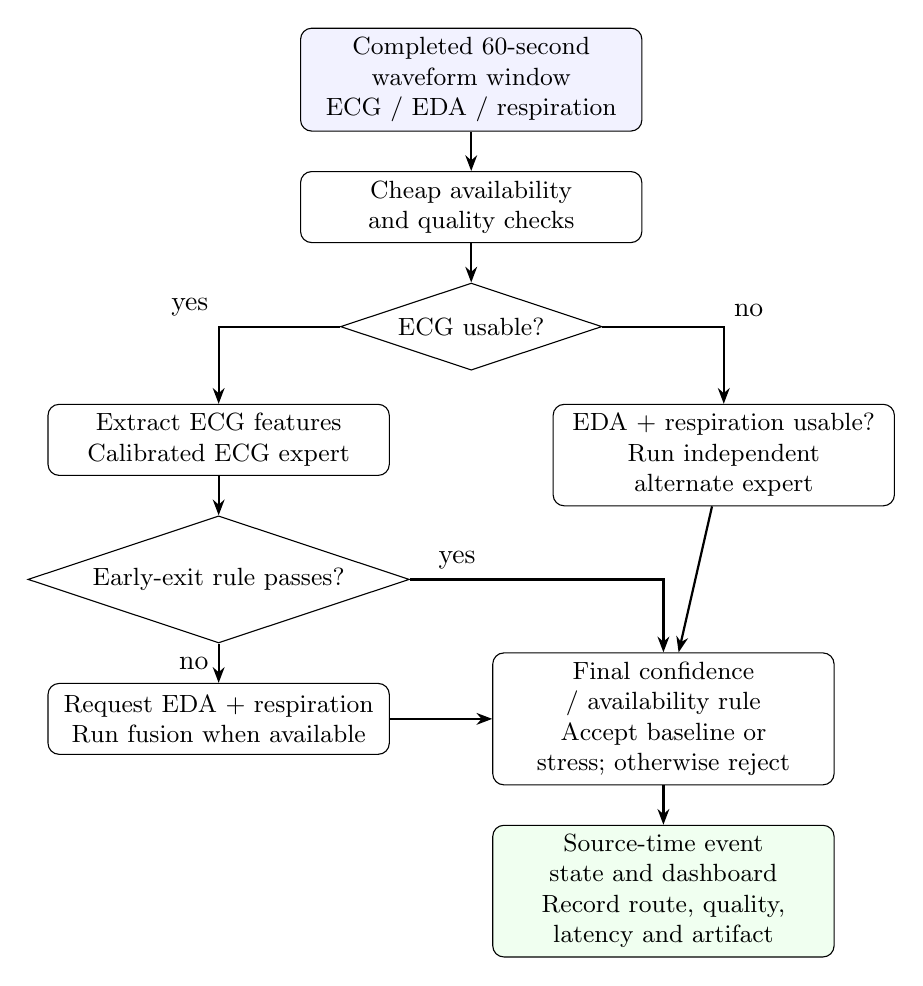
\begin{tikzpicture}[node distance=5mm and 8mm,box/.style={draw,rounded corners,align=center,font=\small,text width=4.1cm,minimum height=9mm},arr/.style={-{Stealth[length=2mm]},thick},choice/.style={draw,diamond,aspect=3,align=center,font=\small,inner sep=1mm}]
\node[box,fill=blue!5] (input) {Completed 60-second waveform window\\ECG / EDA / respiration};
\node[box,below=of input] (qa) {Cheap availability and quality checks};
\node[choice,below=of qa] (usable) {ECG usable?};
\node[box,below left=7mm and 2mm of usable] (ecg) {Extract ECG features\\Calibrated ECG expert};
\node[box,below right=7mm and 2mm of usable] (alt) {EDA + respiration usable?\\Run independent alternate expert};
\node[choice,below=of ecg] (exit) {Early-exit rule passes?};
\node[box,below=of exit] (fuse) {Request EDA + respiration\\Run fusion when available};
\node[box,right=13mm of fuse] (final) {Final confidence / availability rule\\Accept baseline or stress; otherwise reject};
\node[box,below=of final,fill=green!6] (display) {Source-time event state and dashboard\\Record route, quality, latency and artifact};
\draw[arr] (input)--(qa);\draw[arr] (qa)--(usable);
\draw[arr] (usable)-|node[above left]{yes}(ecg);\draw[arr] (usable)-|node[above right]{no}(alt);
\draw[arr] (ecg)--(exit);\draw[arr] (exit)--node[left]{no}(fuse);
\draw[arr] (fuse)--(final);\draw[arr] (alt)--(final);
\draw[arr] (exit.east)--++(6mm,0)node[above]{yes}-|(final.north);
\draw[arr] (final)--(display);
\end{tikzpicture}
\caption{Implemented decision flow. If fusion is unavailable after a usable ECG requests more evidence, the final ECG acceptance rule can still accept it and records that limited-modality reason. Failed ECG requires usable alternate channels; total dropout is rejected. Features already computed within a window are cached.}
\label{fig:routing}
\end{figure*}

\subsection{Data Collection and Window Construction}
The project uses the official WESAD archive and verifies its published checksum before import. The implemented channels are chest ECG, EDA and respiration at 700~Hz. Acceleration is exported as movement context and is not a stress label or an expert input. Wrist BVP, temperature and EMG were part of the broader Evaluation 1 discussion but are outside this implementation's feature schema.

Two tables serve different purposes. The classification table contains 445 nonoverlapping 60-second windows drawn within continuous pure-condition segments: 285 baseline and 160 stress. These reproduce the original seven-feature experiment. The chronological replay uses a separate recording-aligned grid and contains 1,442 windows: 282 baseline, 152 stress and 1,008 mixed or unsupported intervals. The latter retain a missing binary target and remain unscored for binary accuracy; they are not relabeled baseline. Consequently, 434 replay windows are eligible for the primary classification result. This difference in counts follows from window alignment and inclusion rules, not an undocumented removal of difficult predictions.

Each row preserves participant, recording, source file, sample boundaries, start/end seconds and condition metadata. The adapter checks archive entries and recording lengths. Source intervals make replay resets and causal event handling possible and permit a prediction to be traced back to the waveform. Condition labels are used for offline fitting and evaluation only.

\subsection{Preprocessing and Physiological Features}
Features are extracted from a completed trailing window. Filters operate within that available interval and do not use future windows. ECG begins with the original amplitude summaries and adds short-window beat statistics. A causal 5--25~Hz bandpass, squared-energy smoothing and a refractory interval provide an energy-peak detector. RR intervals outside 0.3--2.0~s are excluded; insufficient valid intervals cause an extraction failure. Successive differences only connect adjacent valid RR intervals. The SDNN-style feature is the sample standard deviation of accepted RR intervals, and RMSSD is the root mean square of successive interval differences. These estimates are research features rather than clinically validated normal-beat annotations.

EDA processing uses causal low-pass filtering, downsampling to approximately 10~Hz and a tonic/phasic separation to derive level, slope and response proxies. Respiration uses a causal 0.08--0.70~Hz bandpass and cycle detection. The EDA response measure is a documented proxy, and short-window variability estimates are not treated as diagnostic quantities. Table~\ref{tab:features} gives the fixed feature order. Offline preparation and runtime inference share the same functions, reducing discrepancies between training and replay.

\begin{table}[t]
\centering\small
\caption{Implemented expert inputs. Full fusion contains 20 features. Quality values and participant identifiers are not classifier inputs.}
\label{tab:features}
\begin{tabularx}{\columnwidth}{P{1.2cm}Y}\toprule
Modality & Features\\\midrule
ECG (12) & Mean, standard deviation, minimum, maximum, median, skewness, kurtosis; heart rate, beat count, median RR, SDNN and RMSSD.\\
EDA (5) & Mean, standard deviation, slope, response-rate proxy and phasic standard deviation.\\
Resp. (3) & Cycle rate, interval standard deviation and filtered amplitude standard deviation.\\\bottomrule
\end{tabularx}
\end{table}

\subsection{Signal Quality and Availability}
Quality inspection tests missing fraction, flatline behavior, repeated-extrema clipping proxies, minimum duration and beat/cycle validity. A failed modality is represented as unavailable rather than imputed into a plausible normal waveform. For new v2 bundles, ECG also uses lag-one roughness
\begin{equation}
q_{\mathrm{rough}}=\frac{\frac{1}{N-1}\sum_{i=1}^{N-1}(x_{i+1}-x_i)^2}{\max(2\operatorname{Var}(x),10^{-24})}.
\label{eq:roughness}
\end{equation}
An engineering threshold of 0.5 flags high-frequency corruption in the current 700~Hz ECG setting. The ratio is insensitive to simple multiplicative amplitude scaling, which is useful for the quality check but does not make the classifier's amplitude features invariant. Missing, clipping and roughness thresholds are fixed heuristics, not validated clinical quality annotations. Movement alone is not used to conclude that a person is stressed or a measurement is corrupt.

\begin{figure}[t]
\centering
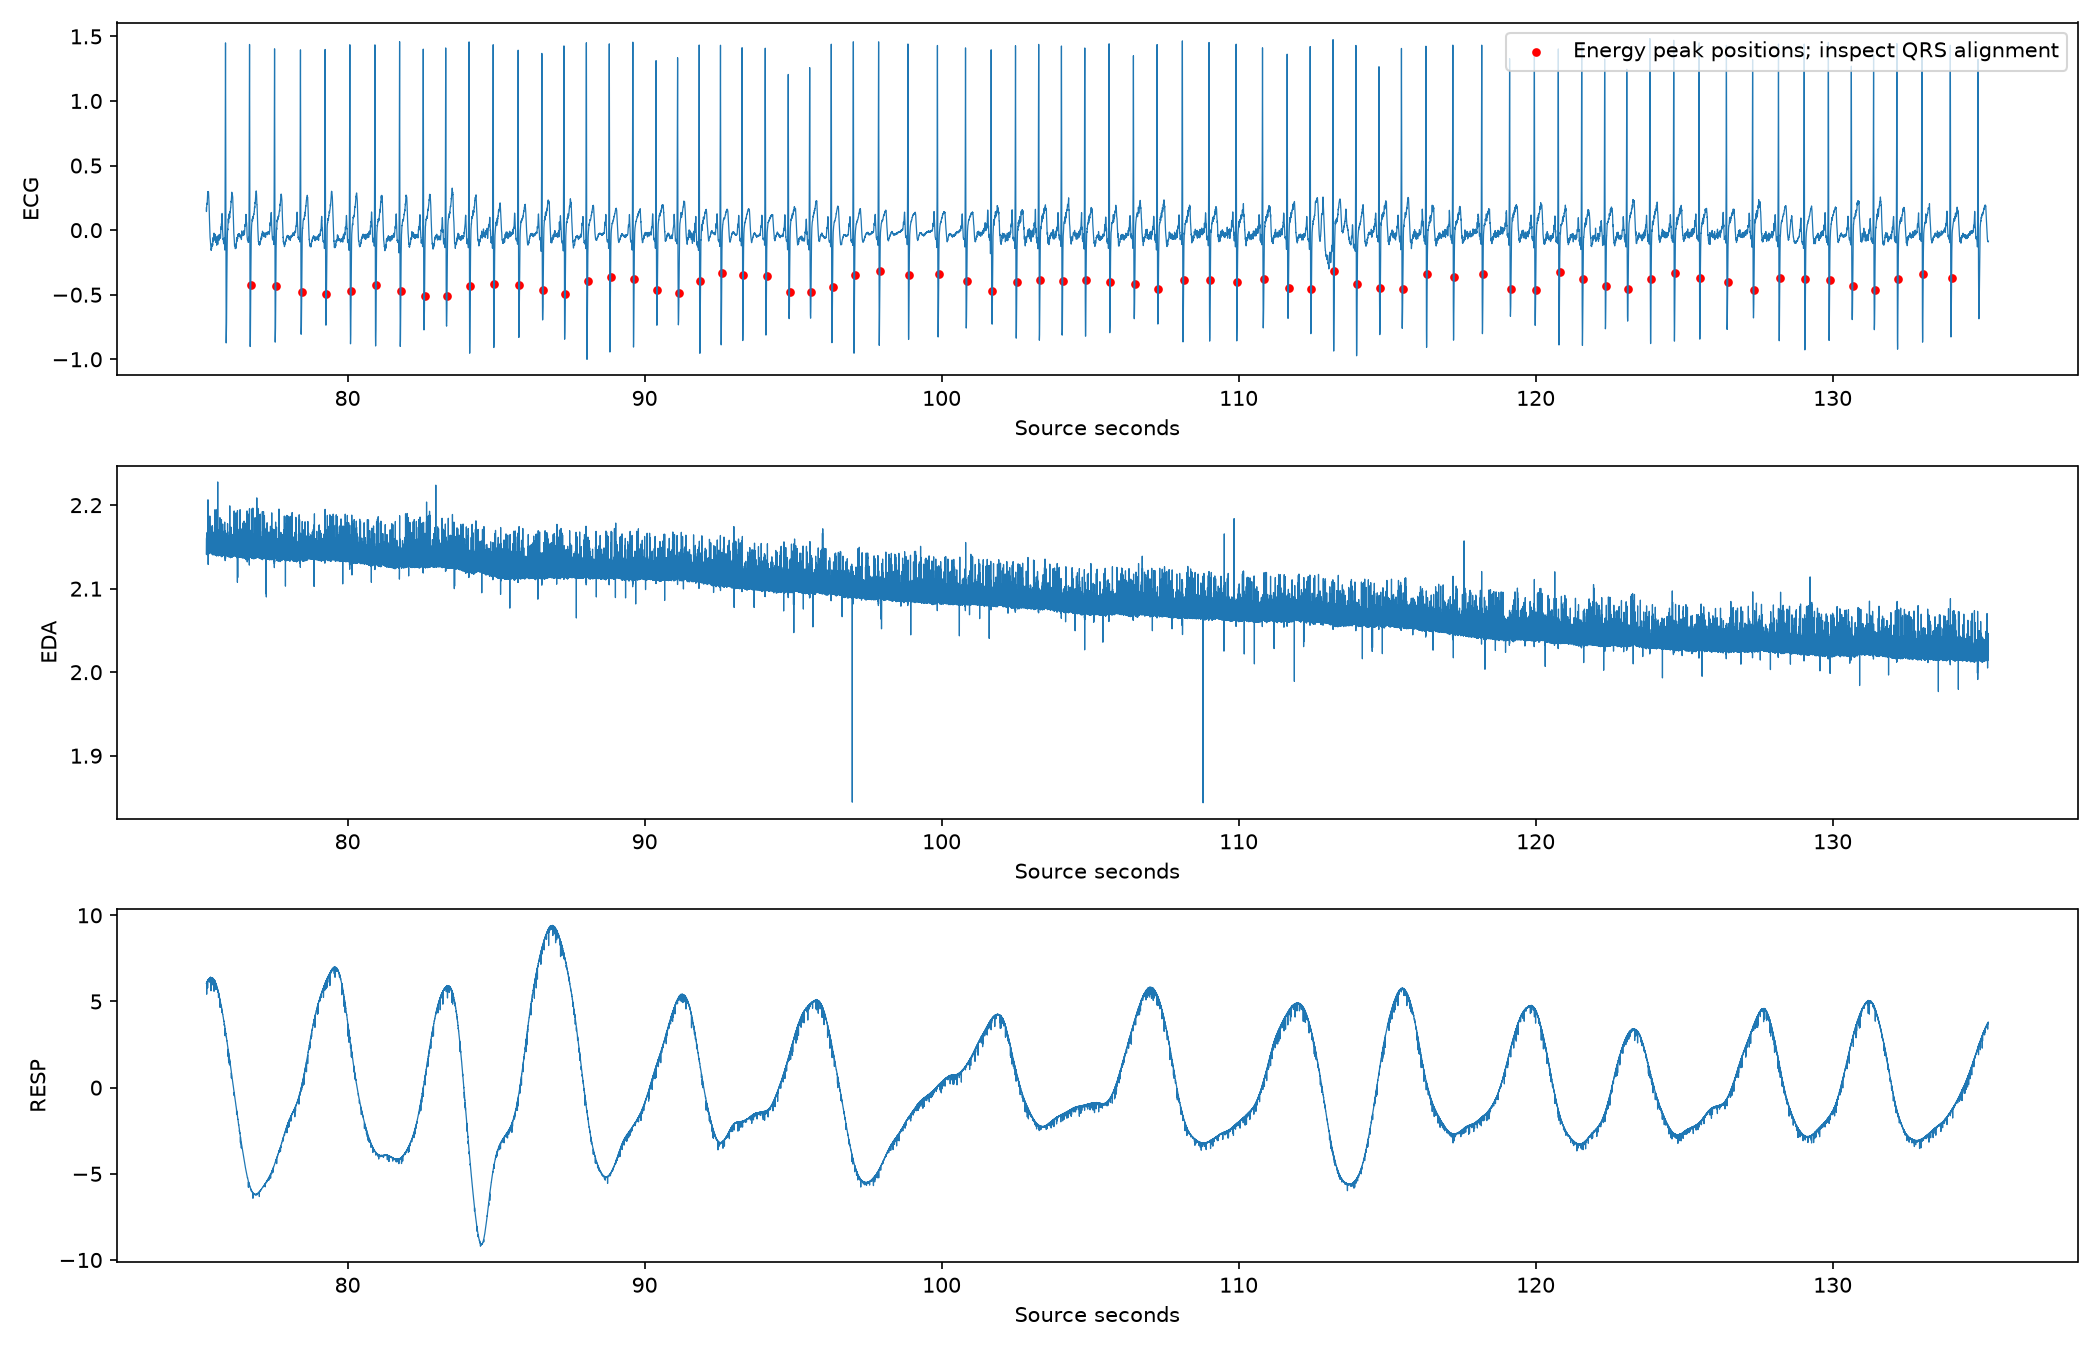
\includegraphics[width=\columnwidth]{waveform_diagnostic.png}
\caption{Qualitative waveform/peak inspection exported from fitting participant S9. This diagnostic checks the plausibility of the processing pipeline; it is not an annotated peak-detection benchmark or held-out accuracy result.}
\label{fig:waveforms}
\end{figure}

\subsection{Expert Models and Participant Separation}
Three experts are fitted: ECG-only, alternate EDA/respiration, and full ECG/EDA/respiration fusion. Candidate families are balanced logistic regression, an RBF SVM and a 100-tree random forest. The revised grouped search also considers SVMs with $C=10$ and either scale-based or 0.01 gamma, plus a compact 64-tree forest with maximum depth six and minimum leaf size three. Median imputation and scaling are fitted in the estimator pipeline; tree models omit scaling. Usability checks require finite supported features before expert inference.

Within each outer development set, participants are assigned to fitting, calibration and policy roles. Inner grouped cross-validation selects expert configurations using mean participant balanced accuracy. A separate participant set fits a sigmoid mapping from decision scores to stress probabilities. The policy participants then select routing thresholds. The outer held-out participant enters none of these stages. The separately fitted final bundle uses nine fitting, three calibration and three policy participants. Group separation is deliberate, but the small number of independent people limits the stability of calibration and policy estimates.

\subsection{Adaptive Decision Making}
Let $p_E$ be the calibrated ECG stress probability. Class-specific early exits use thresholds $\tau_0^{\mathrm{exit}}$ and $\tau_1^{\mathrm{exit}}$:
\begin{equation}
\operatorname{exit}(p_E)=
\begin{cases}
1,&p_E<0.5\ \land\ 1-p_E\geq\tau_0^{\mathrm{exit}},\\
1,&p_E\geq0.5\ \land\ p_E\geq\tau_1^{\mathrm{exit}},\\
0,&\text{otherwise.}
\end{cases}
\end{equation}
When ECG passes this rule, its result is accepted. An uncertain usable ECG requests fusion. Failed ECG requests the independent alternate expert, which has not been trained with invented ECG values. Final acceptance uses separate class-confidence thresholds. If a usable ECG requests fusion but alternate channels are unavailable, ECG can still pass its final acceptance rule; the decision records this reason. Total sensor dropout cannot produce an accepted class.

Development search considers exit thresholds in $\{0.5,0.6,0.7,0.8,0.9,0.95,0.99,1.0\}$ and final thresholds in $\{0.5,0.6,0.7\}$, with exits at least as strict as final acceptance. Among feasible candidates, selection minimizes escalation, then operational error. Constraints require at least 80\pct{} overall and stress coverage, pooled and participant-macro stress recall within three points of the full-evidence reference, and operational error within three points of that reference. They apply to clean and combined development scenarios. Rejection counts as an operational error for this search. Infeasibility is recorded explicitly.

The reference uses fusion when supported, alternate evidence for failed ECG and usable ECG when fusion is unavailable. Development corruption comprises ECG missing bursts, moderate ECG noise and EDA dropout; held-out tests include additional failures and severity. This procedure minimizes an escalation proxy, not measured energy or CPU cost. That distinction becomes important in the final-artifact benchmark.

\subsection{Temporal Decisions and User Notification}
Accepted window decisions feed a causal event tracker with opening confirmation, recovery and cooldown settings selected on policy participants. Participant changes, session changes, gaps, replay restarts and rejected windows clear incompatible evidence. Manual predictions do not accumulate temporal state. Unsupported conditions still pass through the runtime, but their missing binary labels prevent unsupported accuracy claims.

The dashboard displays the window decision, selected expert, quality reasons, probability and processing time. History exports retain source intervals and artifact identity. The event state is kept distinct from a window prediction: a classifier result is not automatically an alert. Evaluation 2 implements this controller but finds weak new-onset detection, so reliable episode alerting is not claimed.

\subsection{Local, Edge and Cloud Interaction}
All implemented inference runs locally. The prototype sends no raw physiological data to a cloud model for its basic decision path. Optional future storage or model-update services would be separate interfaces. The current work therefore demonstrates cloud-independent software execution, while reductions in transmitted bytes, radio energy and battery consumption remain unmeasured. A physical edge device and live sensor link are future integration steps.

\section{Implementation and Experimental Setup}
\subsection{Software and Reproducibility}
The pipeline uses Python 3.14, NumPy, SciPy, pandas, scikit-learn 1.9.1, joblib and Streamlit. The measured host is an arm64 macOS system; its timings are host results rather than Raspberry Pi or wearable measurements. Single-thread limits are applied during evaluation and benchmarking. Versioned outputs retain dataset/code hashes, seeds, participant roles, model parameters, calibrated experts and held-out predictions. The original feature CSV, saved model and historical figures are preserved.

Forty-one automated tests cover signal behavior, modality failures, routing, participant separation, archive handling, temporal resets and the dashboard. A subsequent dashboard check exercised the completed v2 artifact. Exact number macros and tables in this report are generated from saved experiment files; no additional test-set threshold selection is used to prepare the paper. The public dataset is used under its scientific, non-commercial research terms with attribution.

\subsection{Outer Evaluation and Baselines}
Leave-one-subject-out evaluation trains on fourteen participants and scores the remaining participant, repeated for all fifteen. Fitting uses the 445 pure-condition windows; scoring uses the 434 eligible replay windows. All methods receive the same outer source intervals. Original-feature logistic, SVM and forest baselines are fitted on the outer development participants; calibrated experts reserve development participants for calibration and policy selection. Thus comparisons assess complete training procedures with different internal allocations, rather than isolating model family alone.

Ablations include physiological ECG, confidence-only routing, routing without final abstention, always-on fusion and a single-window temporal variant. Clean confidence-only and full-quality decisions coincide because the clean eligible signals pass the quality checks. Their identical clean classification scores should not be interpreted as evidence that quality gates improve clean discrimination.

\subsection{Waveform Failures and Metrics}
The eleven fixed scenarios are clean input; a 25\pct{} ECG missing burst; ECG flatline; ECG clipping; moderate and severe Gaussian ECG noise at 0.5 and 2.0 times the window standard deviation; ECG amplitude scaling by three; EDA dropout; respiration dropout; combined alternate dropout; and total dropout. Perturbations have deterministic row/scenario seeds and precede extraction. Their labels remain the original condition labels. Synthetic corruption supplies controlled failure evidence, not a replacement for annotated real-world artifacts.

For accepted decisions, accuracy, precision and F1 use their standard confusion-count definitions. In addition, accepted coverage and all-window stress recall are
\begin{align}
C&=\frac{N_{\mathrm{accepted}}}{N_{\mathrm{eligible}}},\\
R_{\mathrm{all}}&=\frac{TP_{\mathrm{accepted}}}{N_{\mathrm{eligible\ stress}}}.
\end{align}
Consequently, rejecting a stress window does not remove it from the recall denominator. Balanced accuracy, Brier score, reliability bins and participant bootstrap intervals complement pooled results. Participant-level resampling avoids treating repeated windows as independent people.

\subsection{Processing Benchmarks and Predeclared Targets}
Waveform timing includes quality checks, lazy extraction, expert inference, routing and event updates. It excludes disk input/output, window acquisition and sensor/radio energy. The separate final-bundle benchmark uses 100 representative replay windows, three repeats, four scenarios and independently timed cascade, ECG and fusion paths. It records 300 timings for each mode/scenario combination, startup, model size and process memory. Memory includes the offline participant cache and Python allocator, so it is not a pure streaming device footprint.

The original engineering target was at least 25\pct{} lower mean CPU cost than fusion with at most three percentage points of all-window stress-recall loss, plus clean overall/stress coverage of at least 80\pct{}. Targets are retained unchanged. Point targets are not statistical noninferiority guarantees, and the latency budget for a physical target device remains unevaluated.

\section{Results and Discussion}
\begin{table*}[t]
\centering\caption{Clean participant-held-out results on the same 434 eligible replay windows. All-window recall counts rejected stress as undetected. Accuracy, precision and F1 describe accepted windows; all listed v2 methods have full clean coverage. Baseline CPU was not instrumented and is left unreported.}
\label{tab:clean}\small
\begin{tabular}{lrrrrrrr}\toprule
Method & Acc. (\%) & Bal. acc. (\%) & Prec. (\%) & Recall (\%) & F1 & Cov. (\%) & CPU (ms)\\\midrule
Original ECG logistic & 72.35 & 71.90 & 58.79 & 70.39 & 0.641 & 100.0 & ---\\
Original ECG SVM & 83.18 & 81.14 & 76.87 & 74.34 & 0.756 & 100.0 & ---\\
Original ECG forest & 78.11 & 78.76 & 65.08 & 80.92 & 0.721 & 100.0 & ---\\
Physiological ECG & 85.48 & 82.61 & 83.46 & 73.03 & 0.779 & 100.0 & 11.25\\
Confidence-only cascade & 85.48 & 86.10 & 74.86 & 88.16 & 0.810 & 100.0 & 14.32\\
\textbf{Quality-aware cascade} & 85.48 & 86.10 & 74.86 & 88.16 & 0.810 & 100.0 & 14.24\\
Cascade without abstention & 85.48 & 86.10 & 74.86 & 88.16 & 0.810 & 100.0 & 14.23\\
Always-on fusion & 88.71 & 88.73 & 80.84 & 88.82 & 0.846 & 100.0 & 16.77\\
\bottomrule\end{tabular}
\end{table*}

\subsection{Observation 1: Improved Stress Detection over the ECG Baseline}
The proposed cascade reaches \CascadeAccuracy\pct{} accuracy, \CascadeRecall\pct{} all-window stress recall and \CascadeFone{} stress F1 at full coverage. The original seven-feature ECG SVM obtains 83.18\pct{} accuracy, 74.34\pct{} recall and 0.756 F1 on the same windows. The cascade's gains are 2.30 accuracy points and \RecallGain{} recall points. Figure~\ref{fig:confusion} makes the corresponding counts explicit: it detects 134 of 152 stress windows, compared with the baseline's 113. False stress predictions also increase, from 34 to 45 baseline windows, explaining the precision tradeoff.

\begin{figure*}[t]
\centering
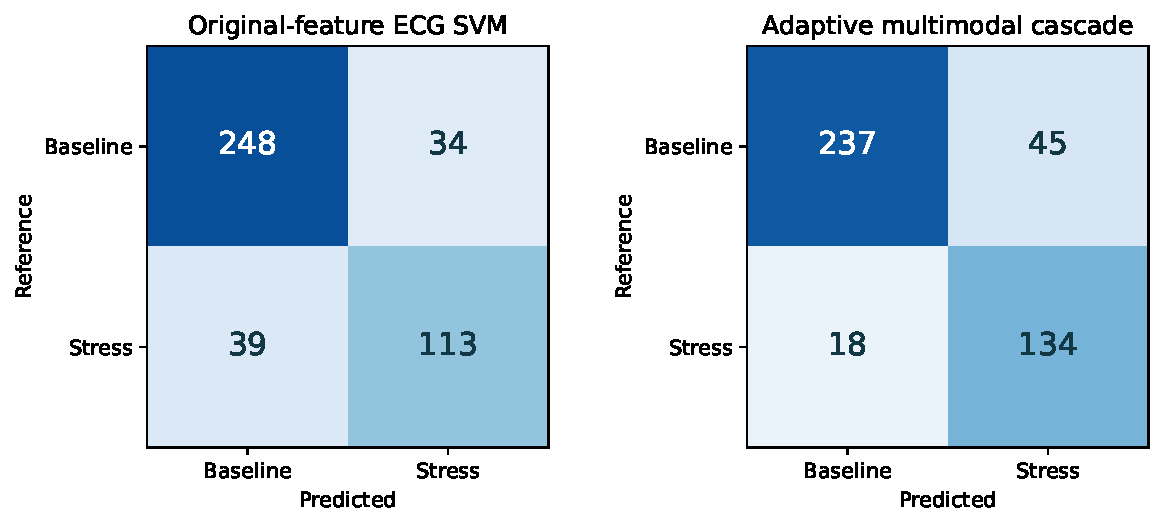
\includegraphics[width=0.85\textwidth]{heldout_confusion.pdf}
\caption{Confusion matrices from the same 434 eligible clean held-out windows. Counts are regenerated from saved row-level predictions. The cascade finds 21 additional stress windows versus the original-feature SVM, with 11 additional false stress predictions. These compare complete training pipelines, not routing in isolation.}
\label{fig:confusion}
\end{figure*}

Relative to the previous v1 cascade, v2 increases recall from 84.21\pct{} to 88.16\pct{} and coverage from 91.47\pct{} to 100\pct{}. However, accepted stress F1 falls from 0.831 to 0.810. The accepted true-stress count rises from 128 to 134 while false stress predictions rise from 32 to 45; the 37 rejected v1 windows are now accepted. These results support improved detection and availability, while showing that full coverage and recall have a false-positive cost.

\subsection{Observation 2: Held-Out Cost--Recall Tradeoff}
Always-on fusion obtains \FusionRecall\pct{} stress recall and 88.71\pct{} accuracy. The adaptive cascade is \RecallGap{} recall points lower while using \CascadeCpu{}~ms mean CPU versus \FusionCpu{}~ms for fusion. The relative saving is
\begin{equation}
S_{\mathrm{CPU}}=1-\frac{T_{\mathrm{cascade}}}{T_{\mathrm{fusion}}}=0.1508.
\end{equation}
Fusion is requested for 37.56\pct{} of the clean scored windows. This is a useful descriptive tradeoff in the held-out training-procedure evaluation: additional processing is avoided on many inputs while most stress detections are retained. It does not imply unchanged overall accuracy or F1. Figure~\ref{fig:tradeoff} includes both gains and regressions across versions.

\begin{figure*}[t]
\centering
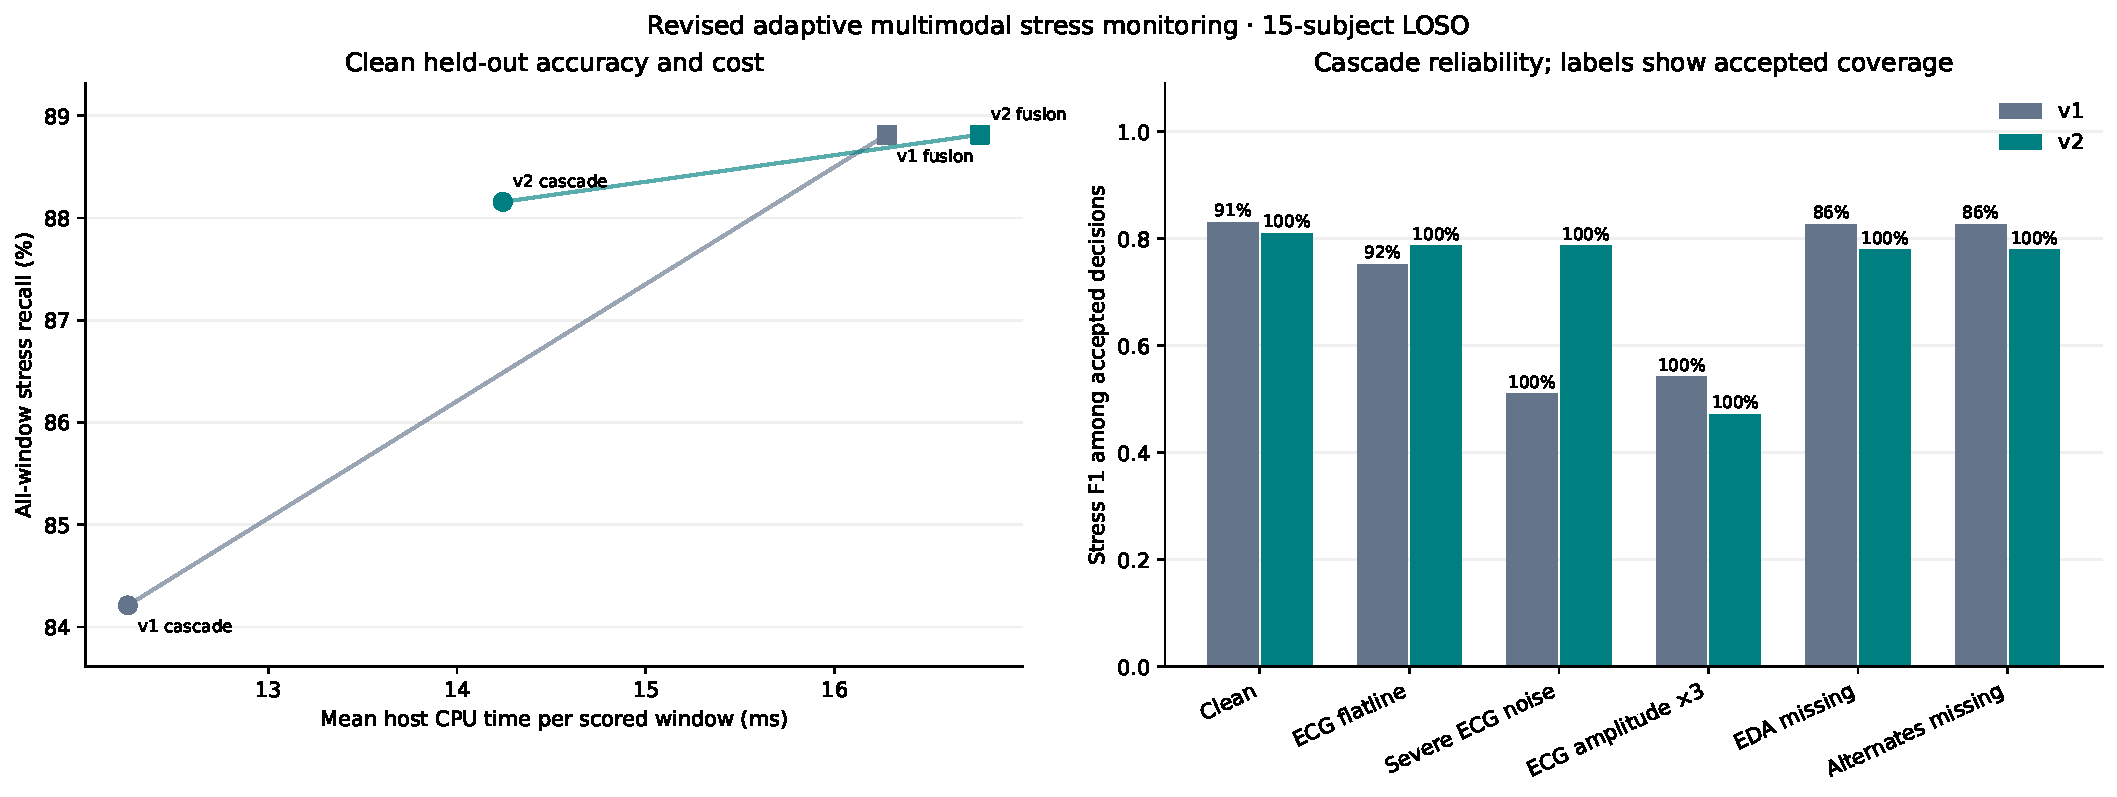
\includegraphics[width=\textwidth]{revision_tradeoff.pdf}
\caption{Verified v1/v2 comparisons. Left: mean host CPU against all-window stress recall on clean scored windows; absolute timing across runs is descriptive. Right: accepted stress F1 under selected scenarios, with coverage labels. Amplitude scaling and alternate-dropout regressions are retained. Full eleven-scenario results are in Table~\ref{tab:failures}.}
\label{fig:tradeoff}
\end{figure*}

The original combined target remains unmet: recall loss now falls within the three-point engineering bound, but CPU saving is below 25\pct{}. This negative result limits the claimed improvement. In addition, the mean participant recall difference versus fusion is $-0.79$ points, with a bootstrap 95\pct{} interval from $-8.67$ to $+5.09$ points. The broad interval does not establish formal noninferiority. Against v1, participant-macro recall changes by $+3.33$ points, with an interval from $-9.33$ to $+20.02$; a pooled improvement alone should not be described as statistically established superiority.

\subsection{Observation 3: ECG-Failure Resilience}
\begin{table*}[t]
\centering\caption{All eleven waveform scenarios: quality-aware cascade compared with the same fold-specific, full-modality-required fusion expert. Acc. and F1 use accepted decisions; recall uses all stress windows. A dash indicates undefined classification quality when coverage is zero. Each scenario has 434 scored windows.}
\label{tab:failures}\small
\begin{tabular}{lrrrrrrrr}\toprule
 & \multicolumn{4}{c}{Adaptive cascade} & \multicolumn{4}{c}{Always-on fusion}\\
Scenario & Cov. (\%) & Acc. (\%) & Rec. (\%) & F1 & Cov. (\%) & Acc. (\%) & Rec. (\%) & F1\\\midrule
Clean & 100.00 & 85.48 & 88.16 & 0.810 & 100.00 & 88.71 & 88.82 & 0.846\\
ECG missing burst & 100.00 & 85.25 & 77.63 & 0.787 & 0.00 & --- & 0.00 & ---\\
ECG flatline & 100.00 & 85.25 & 77.63 & 0.787 & 0.00 & --- & 0.00 & ---\\
ECG clipping & 100.00 & 72.12 & 70.39 & 0.639 & 56.68 & 45.93 & 46.71 & 0.516\\
Moderate ECG noise & 100.00 & 70.97 & 94.74 & 0.696 & 100.00 & 76.96 & 96.05 & 0.745\\
Severe ECG noise & 100.00 & 85.25 & 77.63 & 0.787 & 0.00 & --- & 0.00 & ---\\
ECG amplitude $\times3$ & 100.00 & 57.60 & 53.95 & 0.471 & 100.00 & 57.37 & 93.42 & 0.606\\
EDA dropout & 100.00 & 85.48 & 73.03 & 0.779 & 0.00 & --- & 0.00 & ---\\
Respiration dropout & 100.00 & 85.48 & 73.03 & 0.779 & 0.00 & --- & 0.00 & ---\\
Both alternates dropped & 100.00 & 85.48 & 73.03 & 0.779 & 0.00 & --- & 0.00 & ---\\
Total sensor dropout & 0.00 & --- & 0.00 & --- & 0.00 & --- & 0.00 & ---\\
\bottomrule\end{tabular}
\end{table*}

When ECG is flatlined, the proposed cascade retains 85.25\pct{} accuracy, 77.63\pct{} stress recall and 0.787 F1 at full coverage through the alternate expert. The ECG-only baseline has no usable ECG input, and the full-modality-required fusion reference cannot run. This comparison demonstrates supported fallback availability; it does not imply that fusion could not be redesigned with its own missing-modality strategy.

Under severe ECG noise, the new roughness check rejects ECG and invokes the same alternate expert. Accuracy, recall and F1 consequently match the flatline case. Relative to v1, severe-noise precision rises from 35.06\pct{} to 79.73\pct{} and F1 from 0.510 to 0.787, while recall falls from 93.42\pct{} to 77.63\pct{}. The gain is fewer false stress predictions rather than greater sensitivity under noise. Under total dropout, all windows are rejected and classification quality is undefined; the system does not manufacture normal predictions.

\subsection{Failure Cases and Ablation Interpretation}
Amplitude scaling is a substantial weakness. Tripling ECG amplitude reduces v2 cascade recall to 53.95\pct{}, even though fusion reaches 93.42\pct{}. Amplitude-dependent ECG features shift, and confident early errors can prevent fusion from being consulted. The scale-invariant quality ratio in Eq.~\ref{eq:roughness} does not solve this classifier-distribution problem. A future revision should evaluate scale-robust features and more reliable escalation under distribution change.

EDA, respiration and combined alternate dropout retain full cascade coverage but reduce recall to 73.03\pct{}, below v1's 78.29\pct{}. The system remains operational through ECG, but availability must not be confused with preserved accuracy. Moderate noise and clipping show improvements in the reported recall/F1 tradeoff, while the complete scenario table prevents a few favorable examples from becoming a universal robustness claim.

On clean data, confidence-only, quality-aware and no-final-abstention variants produce identical classifications at the selected v2 operating points. Thus clean results support the integrated adaptive pipeline, whereas evidence for quality gating comes from corrupted inputs. All v2 clean final thresholds are permissive enough to yield full coverage; rejection remains necessary for unsupported measurement failures.

\subsection{Final Fitted Artifact and Host Benchmark}
The final dashboard bundle has artifact identifier \texttt{dae3a7c563c9} and occupies 76,313 bytes, approximately 74.5~KiB. It contains logistic ECG, a compact 64-tree alternate expert and a 100-tree fusion expert. Its calibration and policy participants differ from those of each outer fold. The final early-exit confidence thresholds are 0.9 for baseline and 0.6 for stress, with final acceptance thresholds of 0.5.

On the separate 100-window clean replay benchmark, this fitted cascade averages 19.83~ms CPU versus fusion's 19.65~ms, with 83\pct{} escalation; its p95 total processing is 27.99~ms. It therefore demonstrates no CPU saving on that workload. Restricting existing timings to eligible binary intervals also shows no saving: 29 unique windows and 87 repeat samples per mode yield 20.97~ms for cascade versus 20.07~ms for fusion. The fold-level \CpuSaving\pct{} saving must not be attached to this artifact as a deployment result.

This discrepancy exposes two implementation limits. Policy selection minimizes escalation frequency rather than actual measured processing cost, and a policy fitted to only three participants can transfer poorly to the replay distribution. Expert selection also prioritizes classification score; in the final fusion search the compact and 100-tree forests tie in validation score, but the existing tie order selects the latter. Future selection should compare measured cost at a specified accuracy tolerance. This is an identified next step, not an improvement already demonstrated here.

\subsection{Dashboard and Implementation Evidence}
Figures~\ref{fig:prediction} and~\ref{fig:monitoring} are actual screenshots of the running local application using the completed v2 artifact. The prediction view displays a selected stored window and its inference route. Monitoring advances along source recording time, can be paused, stops at recording completion and resets state when the participant or session changes. History retains quality, route, source interval and model identity. The screenshots demonstrate functionality on participant S10, which is in the final artifact's calibration set; they are not held-out evaluation evidence. Their single displayed processing times are illustrative UI measurements and do not replace the controlled benchmark.

\begin{figure*}[p]
\centering
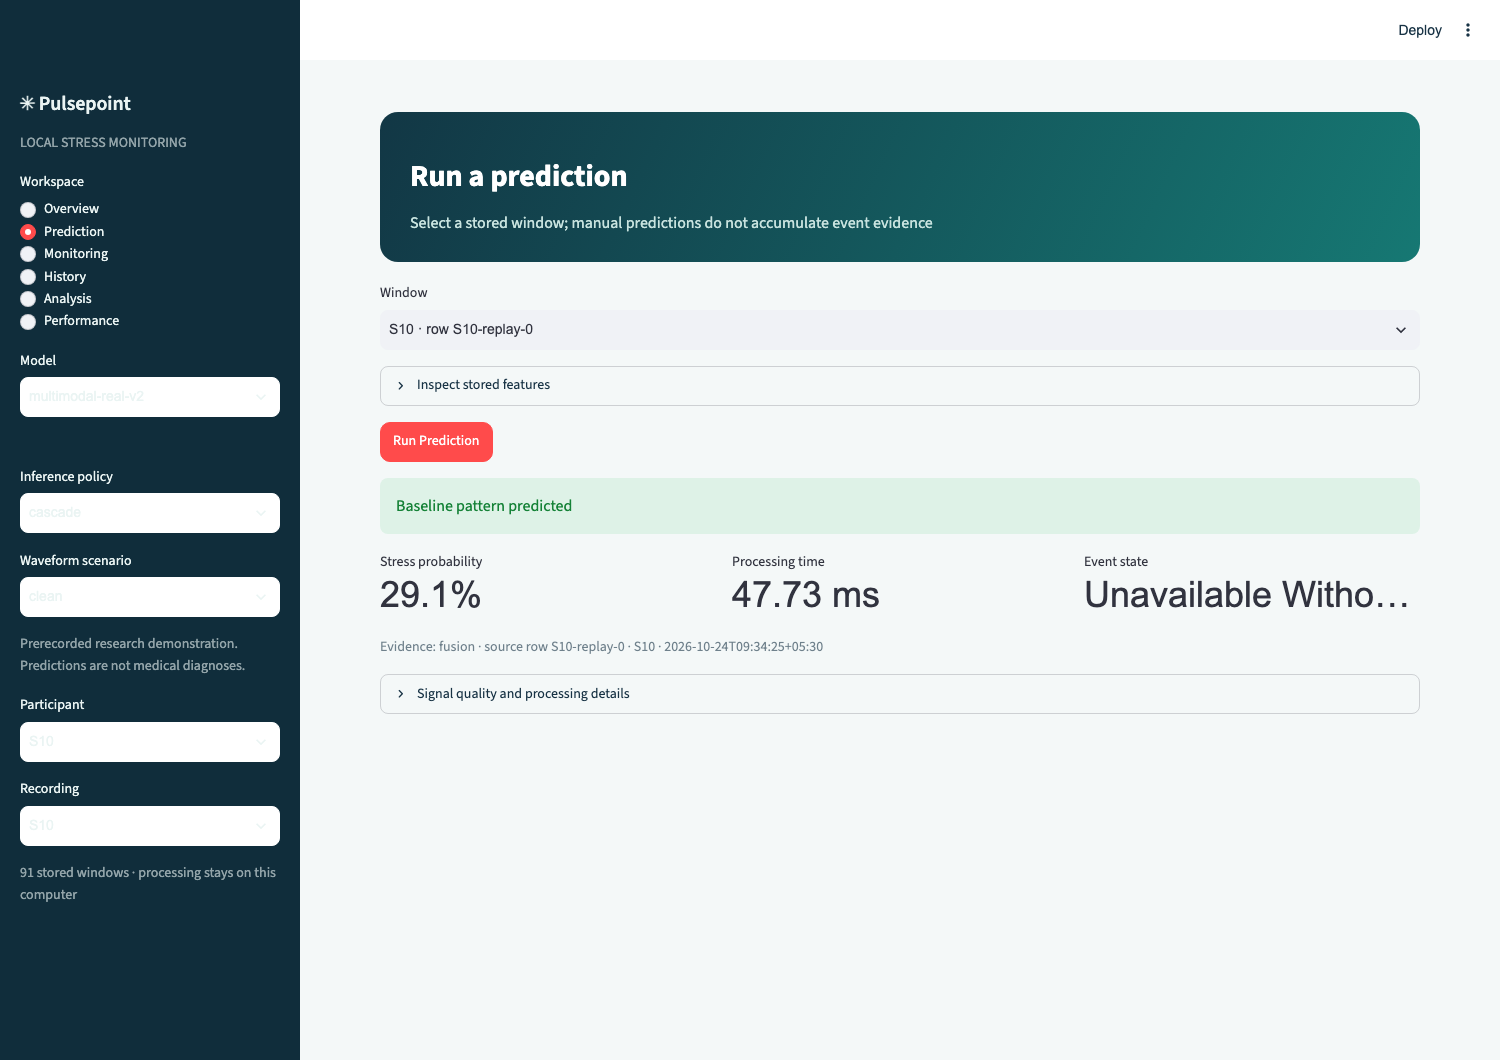
\includegraphics[trim=0 240bp 0 0,clip,width=0.94\textwidth,height=0.37\textheight,keepaspectratio]{dashboard_prediction.png}
\caption{Actual \system{} prediction screenshot using \texttt{multimodal-real-v2}. Capture styling hides local path fields and corrects text contrast; model outputs are not edited. The example is a functional demonstration on S10, not an independent accuracy or latency measurement.}
\label{fig:prediction}
\vspace{4mm}
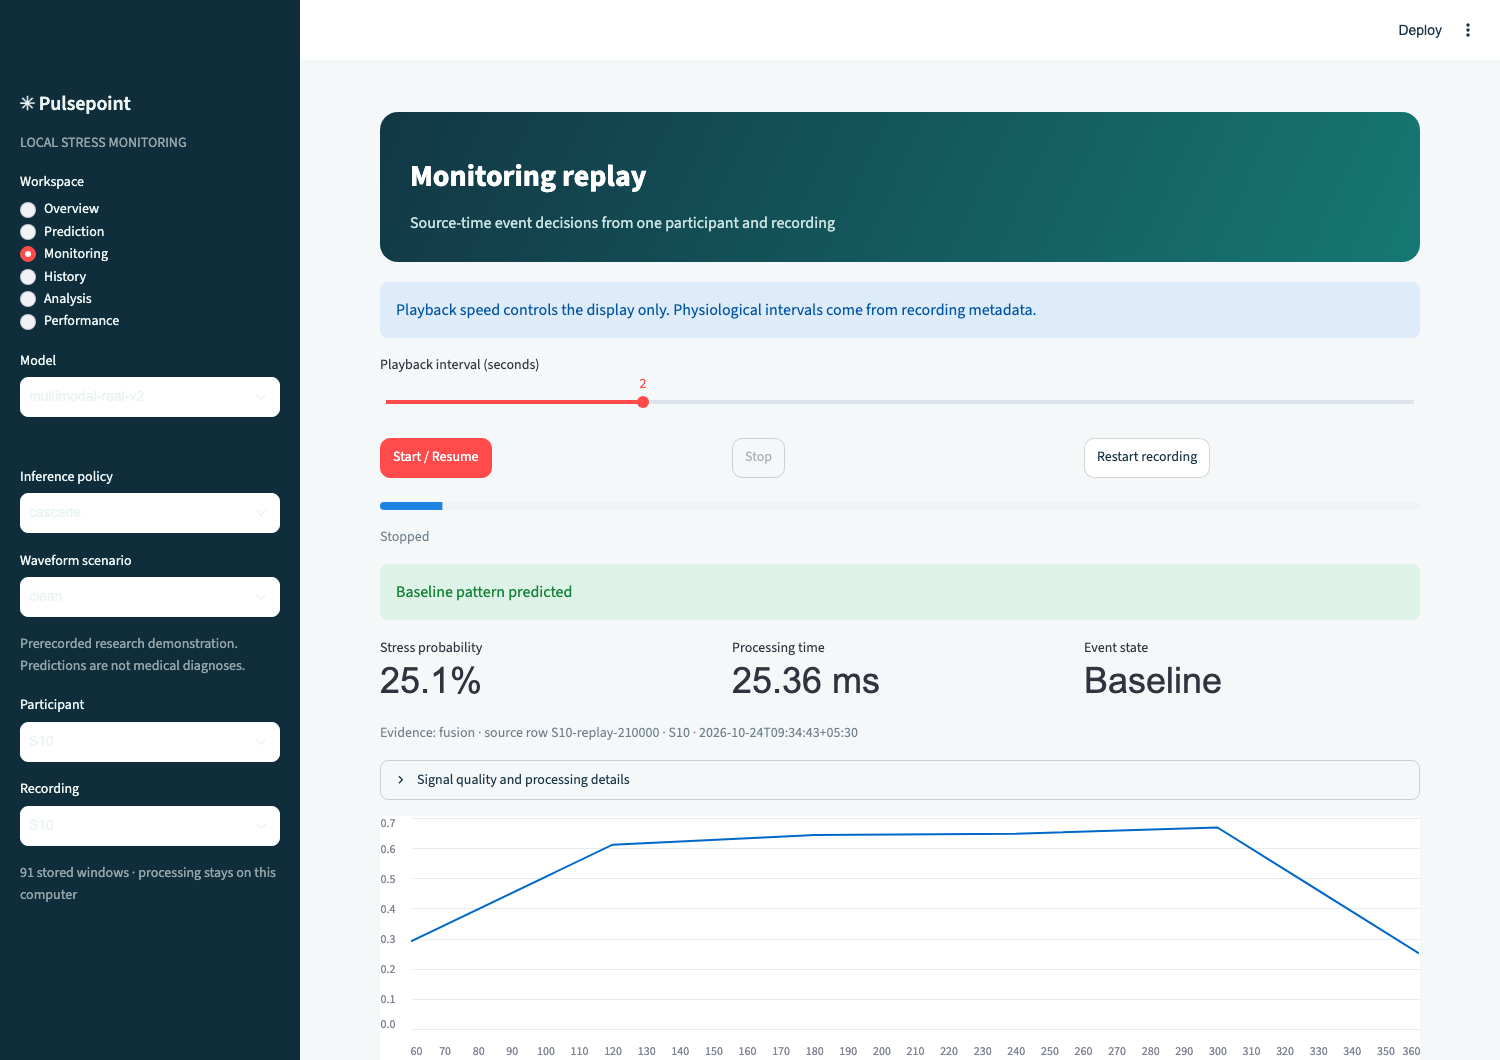
\includegraphics[width=0.94\textwidth,height=0.37\textheight,keepaspectratio]{dashboard_monitoring.png}
\caption{Actual prerecorded monitoring screenshot after source-time replay and pause. The horizontal axis follows recording metadata, and the state tracker remains separate from window classification. This screenshot does not represent a live wearable connection.}
\label{fig:monitoring}
\end{figure*}

\subsection{Temporal Event Findings}
Temporal confirmation reduces new false event starts on eligible baseline time from six for the single-window variant to three. However, only two of fifteen eligible stress episodes receive a new event start with the temporal policy. A state already active before a stress interval is not counted as a newly detected onset. Detection delay is measured from the first fully labeled stress window, rather than the exact condition transition. The low onset count prevents presenting the lower false-start count as reliable event monitoring. Window classification remains the principal positive result of Evaluation 2.

\FloatBarrier
\section{Limitations and Ethical Considerations}
The independent sample consists of fifteen laboratory participants, not hundreds of independent windows. Physiological differences, limited calibration participants and synthetic corruption constrain generalization. The same WESAD cohort has already informed the revision, so participant-disjoint nested evaluation prevents direct fitting leakage within the run but does not create a new confirmatory dataset. The presented improvements are exploratory and require independent replication.

Quality heuristics are conservative engineering checks without clinical artifact labels. The energy-peak detector has synthetic tests and qualitative overlays but no annotated clinical peak-validation study. EDA filter startup can influence response proxies, and short-window HRV estimates are limited. Unsupported replay conditions are processed but not scored as binary baseline or stress. The method therefore does not establish recognition across all affective states or reliable day-long false-alert rates.

The final artifact does not demonstrate processing savings on its benchmark, and the overall 25\pct{} target remains unmet. Host CPU time excludes acquisition, disk input/output and communications. No power instrumentation, physical edge-device deployment, network-traffic comparison or battery experiment was completed. Local processing avoids a cloud dependency in this software path but is not a complete privacy or security guarantee.

The application is a research monitoring prototype, not a medical diagnostic system. False stress and missed stress predictions remain possible. Physiological data and exported histories should be handled according to the dataset's research terms and applicable institutional requirements. No new participant recruitment or clinical validation is claimed in this report.

\section{Future Scope}
The next technical priority is to evaluate ECG features that are robust to sensor-gain changes while preserving meaningful beat information. Routing should also consider evidence that the input differs from development data, rather than relying exclusively on a calibrated probability. Both changes require development-only design and a separately versioned evaluation; changing thresholds until the current test scores improve would weaken the evidence.

Efficiency selection should incorporate actual stage costs and deployment workloads, with a cost-aware tie rule for comparable models. Grouped cross-fitting and a larger independent cohort could improve use of limited data and assess calibration stability. Personalization remains a separate study with an explicit onboarding interval excluded from evaluation.

Live wearable acquisition, Raspberry Pi or microcontroller implementation and instrumented power measurements are natural AIoT integration steps. A CNN, model compression, federated updates and wrist-sensor fusion can be investigated after the current failure modes and hardware constraints are better characterized. These remain future scope from Evaluation 1, not completed features of Evaluation 2.

\section{Conclusion}
This work extends the Evaluation 1 edge-based stress-monitoring proposal into a reproducible quality-aware adaptive multimodal prototype. The literature motivates local inference, complementary sensing, explicit rejection and careful deployment measurement while establishing that adaptive sensing has prior art. The implementation combines calibrated ECG, alternate and fusion experts with independent escalation and acceptance rules, waveform quality checks and a shared local dashboard runtime.

On 434 eligible windows from fifteen held-out WESAD participants, the cascade achieves \CascadeAccuracy\pct{} accuracy and \CascadeRecall\pct{} stress recall at full coverage. It improves stress recall by \RecallGain{} points over the original-feature ECG SVM and reduces mean CPU by \CpuSaving\pct{} relative to fold-specific fusion with a \RecallGap{}-point recall gap. Alternate sensing preserves useful predictions under ECG failure. These are the principal positive observations for Evaluation 2.

The measured tradeoff remains qualified: clean F1 is below fusion, amplitude scaling and alternate dropout expose weaknesses, new-onset event detection is poor, and the separate fitted artifact shows no CPU saving. The original combined efficiency target remains unmet. The completed contribution is a transparent software implementation and laboratory evaluation whose limitations identify the next steps toward reliable physical edge deployment.

\balance
\begin{thebibliography}{00}
\bibitem{schmidt2018} P. Schmidt, A. Reiss, R. D\"urichen, C. Marberger, and K. Van Laerhoven, ``Introducing WESAD, a multimodal dataset for wearable stress and affect detection,'' in \emph{Proc. ACM Int. Conf. Multimodal Interaction (ICMI)}, 2018, pp. 400--408, doi: \href{https://doi.org/10.1145/3242969.3242985}{10.1145/3242969.3242985}.
\bibitem{pereira2024} C. V. F. Pereira, E. M. de Oliveira, and A. D. de Souza, ``Machine learning applied to edge computing and wearable devices for healthcare: Systematic mapping of the literature,'' \emph{Sensors}, vol. 24, no. 19, Art. no. 6322, 2024, doi: \href{https://doi.org/10.3390/s24196322}{10.3390/s24196322}.
\bibitem{mitro2023} N. Mitro \emph{et al.}, ``AI-enabled smart wristband providing real-time vital signs and stress monitoring,'' \emph{Sensors}, vol. 23, no. 5, Art. no. 2821, 2023, doi: \href{https://doi.org/10.3390/s23052821}{10.3390/s23052821}.
\bibitem{fauzi2022} M. A. Fauzi, B. Yang, and B. Blobel, ``Comparative analysis between individual, centralized, and federated learning for smartwatch based stress detection,'' \emph{J. Personalized Medicine}, vol. 12, no. 10, Art. no. 1584, 2022, doi: \href{https://doi.org/10.3390/jpm12101584}{10.3390/jpm12101584}.
\bibitem{amser2022} E. K. Naeini, S. Shahhosseini, A. Kanduri, P. Liljeberg, A. M. Rahmani, and N. Dutt, ``AMSER: Adaptive multimodal sensing for energy efficient and resilient eHealth systems,'' in \emph{Proc. Design, Automation \& Test in Europe Conf. \& Exhibition (DATE)}, 2022, pp. 1455--1460, doi: \href{https://doi.org/10.23919/DATE54114.2022.9774590}{10.23919/DATE54114.2022.9774590}.
\bibitem{geifman2017} Y. Geifman and R. El-Yaniv, ``Selective classification for deep neural networks,'' in \emph{Advances in Neural Information Processing Systems}, vol. 30, 2017. [Online]. Available: \url{https://proceedings.neurips.cc/paper_files/paper/2017/hash/4a8423d5e91fda00bb7e46540e2b0cf1-Abstract.html}
\end{thebibliography}
\end{document}
